After I analyzed the impact on data rate and robustness of physical layer parameter, I will simulate a platooning
scenario in ns-3 to find the influence of the found physical layer configuration on the network performance.
The network performance metric consists of the transmission latency, which describes the time needed to transmit the data
on application layer, and the update rate of the platooning service, which defines how long ago a new position update
was received by the \ac{TM} in the Platooning Service.

Ns-3 is suitable for this simulation, because it supports simulation on the application layer level. Via the extension Netsimulyzer
a graphical user interface to visualize the simulation results is available.

Any packets in ns-3 can be tagged with a packet Tag \footnote{https://www.nsnam.org/docs/release/3.36/doxygen/classns3_1_1_tag.html},
which are designed to add additional information to the packet. Every added packet Tag belongs to the packet and does not change
the packet size or characteristics. Throughout the simulation, I used packets tags to add information, which were needed to be
transferred.

The simulation scenario is based on the corn harvest and loading scenario, which is described in \autoref{sec:corn_harvest_scenario}, where
multiple \ac{FH}s harvest the corn and load it onto one of the \ac{TM}s.

Thereby, every \ac{FH} starts in the lower left corner of the field and harvests the corn along the path,
which is displayed in \autoref{fig:PlatooningRoute}. As soon as a \ac{FH} reaches a field border, it makes a U-turn and continues
in the opposite direction.
Every \ac{FH} harvests the corn until it reaches the end of the field in the lower right corner.
The inital position of the \ac{TMs} is a row below the \ac{FH}s, which is displayed in \autoref{fig:PlatooningInit}.
\begin{figure}[H]%
	\centering
	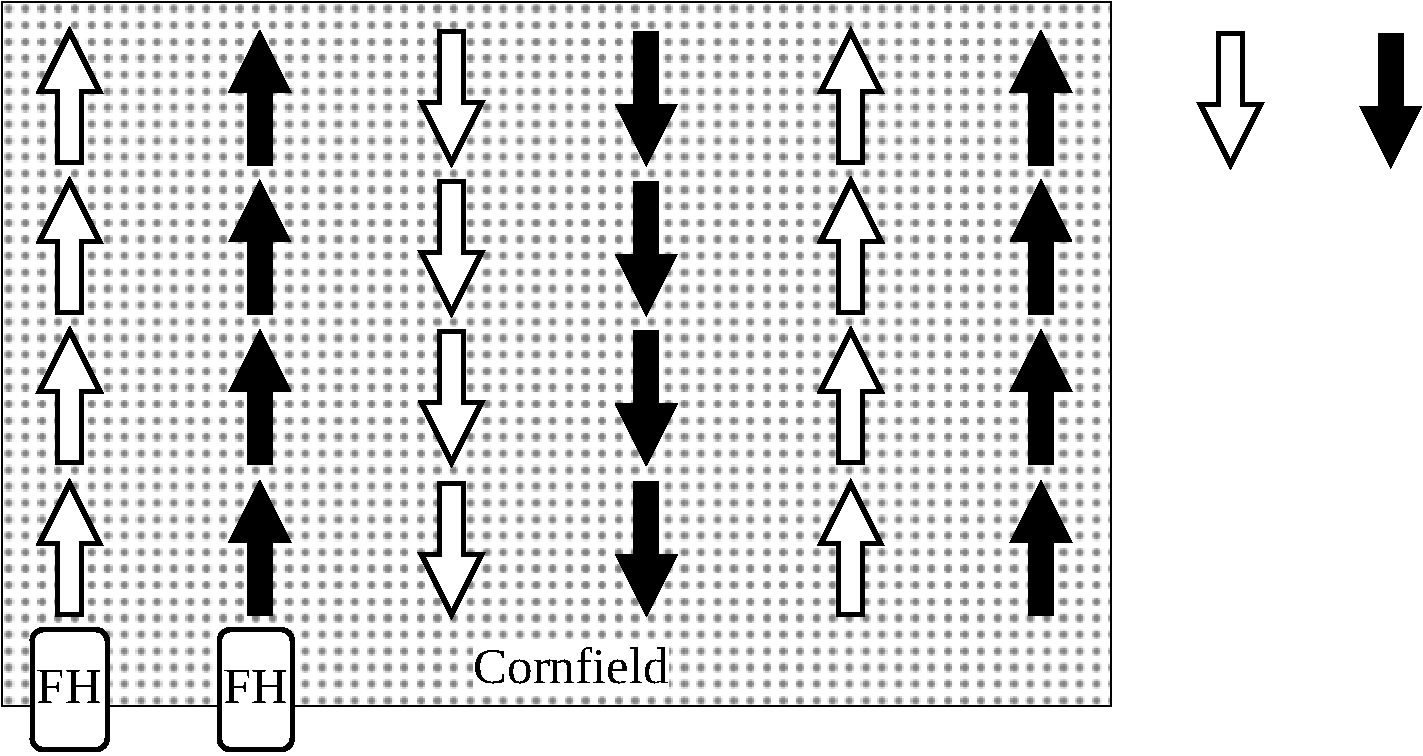
\includegraphics[width=0.7\textwidth]{figures/drawings-Route}
	\caption{Path of the \acf{FH} for harvesting corn on the field}
	\label{fig:PlatooningRoute}%
\end{figure}

Every machine is represented by a ns-3 Node. Each Node has a mobility model, which describes the movement of the machine.
In order to exchange data between the machines, every machine is equipped with ns-3 WifiNetDevice, which is a IEEE 802.11ax
Wi-Fi device. Every Wi-Fi Device runs in Ad-Hoc mode to enable direct communication
between the machines. The Wi-Fi data rate is managed by a Constant Rate Wifi Manager, which has a Non-Uniform
transmission mode and a data mode for uniform transmissions.
The transmission modes are configured according
to the parameters in \autoref{tab:SimulationParametersWiFi}.
The parameters are chosen from the results of the physical layer analysis of
\autoref{sec:DataRate} and \autoref{sec:Robustness}. Non-uniform transmissions are used to broadcast the Agricultural Platooning
Service advertisements. The non-uniform transmission parameters enable the longest possible
transmission range, which results in the lowest data rate. Since no high data rate is required to advertise the Service, the parameters were
chosen to maximize the transmission range. Uniform transmission parameters are used to exchange Agricultural Platooning Service data between
the \ac{FH} and the \ac{TM}. \todo{Robustness?DataRate? Fieldexperiments}

\begin{table}[H]
	\centering
	\begin{tabular}{p{5cm}p{4cm}}
		\toprule
		General Parameters & \\
		\midrule
		Wi-Fi Standard & IEEE 802.11ax\\
		\ac{GI} & \SI{3200}{\nano\second}\\
		Frequency Spectrum & \SI{5.6}{\giga\hertz}\\
		\ac{BW} & \SI{20}{\mega\hertz}\\
		max. Transmission Power & \SI{25}{\dBm}\\
		Antenna Gain & \SI{5}{\dB}\\
		Maximum retries & \num{3}\\
		\midrule
		Uniform Transmission Parameters & \\
		\midrule
		\ac{MCS} & \num{5}\\
		Number \ac{MIMO} Streams & \num{2}\\
		\midrule
		Non-Uniform Transmission Parameters & \\
		\midrule
		Broadcast \ac{MCS} & \num{0}\\
		\ac{ER} mode enabled & True\\
		\ac{DCM} enabled & True\\
		\bottomrule
	\end{tabular}
	\caption{Simulation parameters for Wi-Fi Devices}
	\label{tab:SimulationParametersWiFi}
\end{table}
\todo[color=blue]{new line or vertical lines?}

Every machine node runs a ns-3 Application, which is responsible for the Agricultural Platooning Service. The application
is identified by a unique identifier runs an UDP socket to exchange data with other Agricultural Platooning Service applications.
Every UDP socket can be addressed by a IP address and a port number. The IP address is the IP address of the machine node.

In the beginning, every \ac{FH} broadcasts a search request to find a empty \ac{TM} to load the corn onto.
As shown in \autoref{fig:PlatooningInit}, multiple \ac{TM}s receive the search request and answer with their current fill level of the \ac{TM}'s
trailer. The \ac{FH} chooses the \ac{TM} with the lowest fill level and sends a connection request to the \ac{TM}. As soon as the 
\ac{TM} receives the connection request, it answers with a connection response. When the \ac{FH} receives the connection response, a
Agricultural Platooning Service is started.

Next, the \ac{FH} starts to harvest the corn. The FH harvest process is defined by the harvest states in \autoref{tab:HarvestStates},
where every harvest state represents a different \ac{PD} and \ac{FH} speed. When the \ac{PD} is low, the \ac{FH} can harvest faster
and vice versa.

Starting in the harvest state H1, the \ac{FH} determines the next harvest state every \SI{50}{\milli\second} by the Markov chain in
\autoref{fig:MarkovChain}. This Markov chain ensures that the harvest state can't transverse from H0 to H2 directly, which would represent
a low \ac{PD} immediately followed by a high \ac{PD}. As I have not enough harvest process data, which contain the \ac{PD} and the \ac{FH} speed,
I chose the transition probabilities randomly\todo[color=blue]{by common sense?}.

After determining the next harvest state, the \ac{FH} sets the \ac{PD} and the \ac{FH} speed according to the defined values in
\autoref{tab:HarvestStates}. The position of the \ac{FH} is advanced by the \ac{FH} speed multiplied with \SI{50}{\milli\second} along the
harvest path in \autoref{fig:PlatooningRoute}. The harvested volume during this time step of \SI{50}{\milli\second} is calculated:cd ..


\begin{table}[H]
	\centering
	\begin{tabular}{>{\centering}p{2cm}p{4cm}p{4cm}}
		\toprule
		Harvest State & \ac{PD} & \ac{FH} speed\\
		\midrule
		H0 & \SI{30}{\tonne\per\hectare}
        & \SI{10}{\kilo\metre\per\hour} \\
		H1 & \SI{40}{\tonne\per\hectare}
        & \SI{8}{\kilo\metre\per\hour} \\
		H2 & \SI{50}{\tonne\per\hectare}
        & \SI{6}{\kilo\metre\per\hour} \\
		\bottomrule
	\end{tabular}
	\caption{Corn harvest states, which define a range of \acf{PD}s and \ac{FH} speeds, where the data is based on the
	key figures \cite{faustzahlen2018}}
	\label{tab:markov_chain}
\end{table}

\begin{figure}[H]
\centering
\begin{tikzpicture}[->, >=stealth', auto, semithick, node distance=3cm]
	\tikzstyle{every state}=[fill=white,draw=black,thick,text=black,scale=1]
    \node[circle, draw]    (A)               {H0};
	\node[circle, draw]    (B)[right of=A]   {H1};
	\node[circle, draw]    (C)[right of=B]   {H2};
	\path
	(A) edge[loop left]			node{0.7}	(A)
        edge[bend left,above]	node{0.3}	(B)
	(B) edge[bend left,below]	node{0.2}	(A)
        edge[bend left,above]   node{0.2}	(C)
        edge[loop]		        node{0.6}	(B)
	(C) edge[bend left,below]	node{0.3}	(B)
        edge[loop right]		node{0.7}	(C);
	\end{tikzpicture}
\caption{Markov Chain for the states \acs{PD} 0, 1 and 2, which represent the current \acf{PD} and harvest speed from \autoref{tab:markov_chain}.}
\label{fig:MarkovChain}
\end{figure}



\begin{table}[H]
	\centering
	\begin{tabular}{p{5cm}p{4cm}}
		\toprule
		Parameters & \\
		\midrule
		Broadcast Interval & \SI{1}{\second}\\
		Broadcast Data & \SI{500}{\byte}\\
		Position Service Update Interval & \SI{50}{\milli\second}\\
		Platoon Service Data & \SI{1000}{\byte}\\
		Field Size & \SI{2000}{\meter} x \SI{1000}{\meter}\\
		\bottomrule
	\end{tabular}
	\caption{Simulation parameters for the Application Agricultural Platooning Service}
	\label{tab:SimulationParameters}
\end{table}


\begin{algorithm}
\begin{algorithmic}[1]
\STATE Create packet data $SearchTM$ of length $SearchPacketLength$ bytes
\STATE Broadcast $SearchTM$ to all \acs{TM}s
\IF {no \acs{TM} ansers}
    \STATE Repeat Broadcasting $SearchTM$ every $SearchPacketInterval$ seconds
\ELSE
	\STATE Send connection request
	\IF {No \acs{TM} response}
		\STATE Repeat Broadcasting $SearchTM$ every $SearchPacketInterval$ seconds
	\ELSE
		\STATE Connection established
		\STATE Start Agricultural Platooning Service
	\ENDIF
\ENDIF
\end{algorithmic}
\caption{Procedure to detect packet errors}
\label{alg:SearchTM}
\end{algorithm}

\begin{figure}[H]%
	\centering
	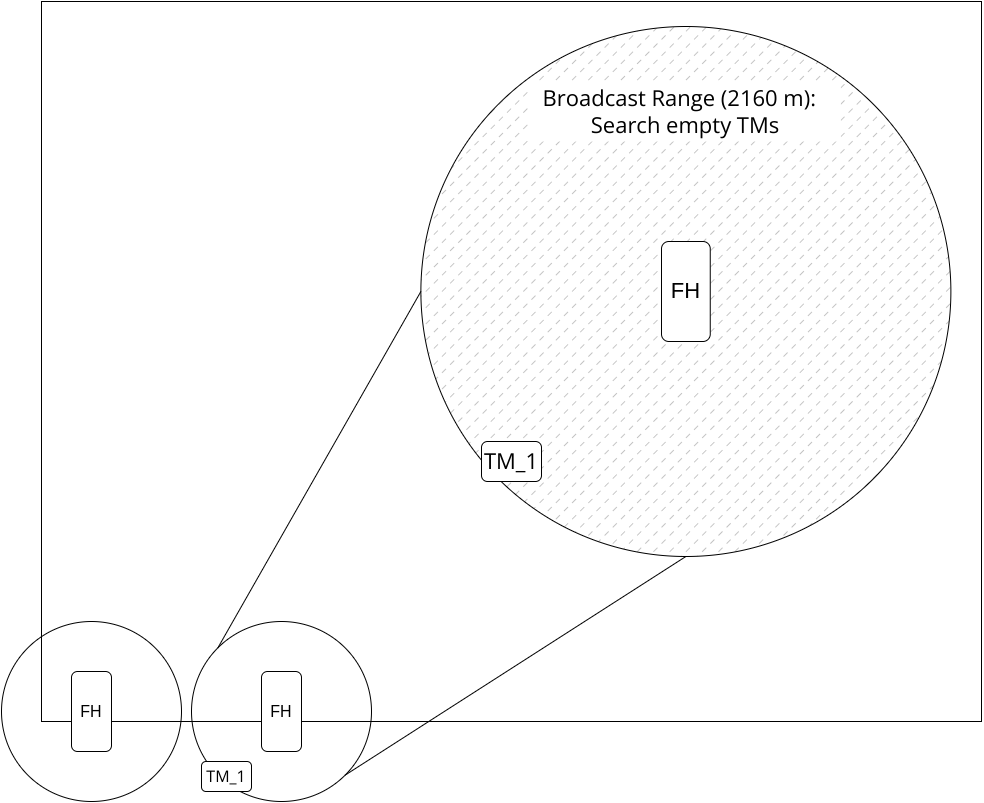
\includegraphics[width=0.7\textwidth]{figures/drawings-INIT}
	\caption{Simulated PER in regards to SNR for chosen HE-MCS values for IEEE 802.11ax physical layer parameters
			of a GI of 3200 ns, a bandwidth of 20 MHz and 2 spatial streams.}
	\label{fig:PlatooningInit}%
\end{figure}

\begin{figure}
\centering
\begin{tikzpicture}[->, >=stealth', auto, semithick, node distance=3cm]
	\tikzstyle{every state}=[fill=white,draw=black,thick,text=black,scale=1]
    \node[circle, draw]    (A)               {Broadcast Search Request};
	\node[circle, draw]    (B)[right, above of=A]   {C};
	\node[circle, draw]    (C)[right of=B]   {H2};
	\path
	(A) edge[loop left]			node{No TM response}	(A)
        edge[bend left,above]	node{0.3}	(B)
	(B) edge[bend left,below]	node{0.2}	(A)
        edge[bend left,above]   node{0.2}	(C)
        edge[loop]		        node{0.6}	(B)
	(C) edge[bend left,below]	node{0.3}	(B)
        edge[loop right]		node{0.7}	(C);
	%\node[above=0.5cm] (A){Patch G};
	%\draw[red] ($(D)+(-1.5,0)$) ellipse (2cm and 3.5cm)node[yshift=3cm]{Patch H};
	\end{tikzpicture}
\caption{Markov Chain for the states \acs{PD} 0, 1 and 2, which represent the current \acf{PD} and harvest speed from \autoref{tab:markov_chain}.}
\label{fig:ConnectionStates}
\end{figure}


\textcite{zhang_method_2009} defined a data frame of \SI{32}{\byte}, which includes an identifier, timestamp, Longitude, Latitude, Heading, Speed and Direction.
Diese Menge an Daten umfasst eine Grundmenge, welche für die Umsetzung eines Platooning Services ausreichen kann, wie die Autoren zeigen.
\textcite{schlingmann_aef_2019} spezifizieren die Datenmenge nicht weiter und weißen darauf hin, dass die benötigte Datenrate für Platooning Services gering ist.

Ich habe für die Simulation von Platooning Services die Datenmenge auf \SI{1}{\kilo\byte} gesetzt. Diese Datengröße ist eine Abstrahierung des Speicherplatzes, welcher möglicherweise für zusätzliche Daten oder Implementierungen von Authentifizierung -  und Sicherheitsmechanismen benötigt wird. Im Corn Harvest scenario können zusätzliche Daten z.B. der Füllstand der Transportmachine sein. 


Service Discovery

Rebroadcast by Count?
additional Traffic

MANET Service discovery

Visualisierung Netsimulyzer

Farbcodes

\begin{figure}[H]%
	\centering
	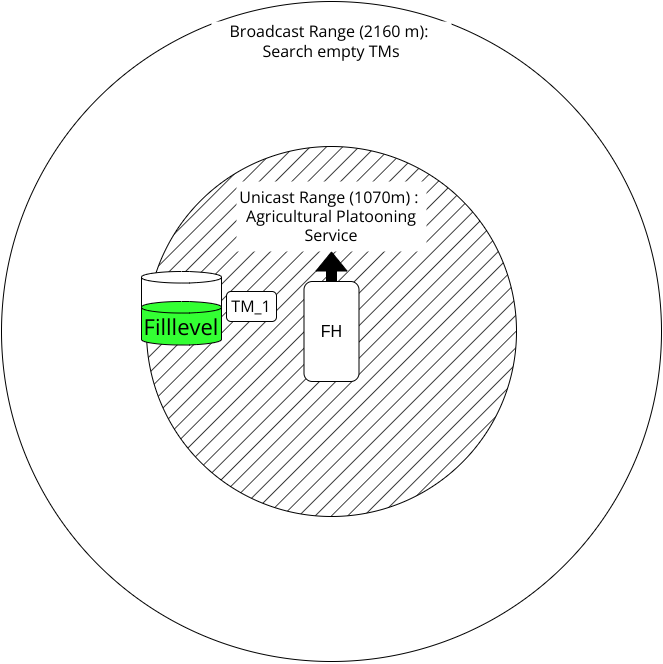
\includegraphics[width=0.7\textwidth]{figures/drawings-HALF_Full}
	\caption{Simulated PER in regards to SNR for chosen HE-MCS values for IEEE 802.11ax physical layer parameters
			of a GI of 3200 ns, a bandwidth of 20 MHz and 2 spatial streams.}
	\label{fig:PlatooningHF}%
\end{figure}

\begin{figure}[H]%
	\centering
	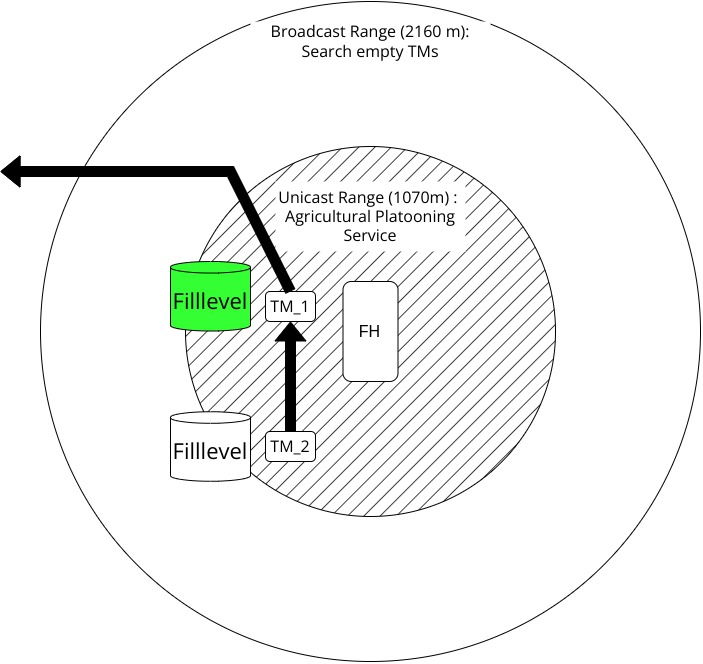
\includegraphics[width=0.7\textwidth]{figures/drawings-FULL}
	\caption{Simulated PER in regards to SNR for chosen HE-MCS values for IEEE 802.11ax physical layer parameters
			of a GI of 3200 ns, a bandwidth of 20 MHz and 2 spatial streams.}
	\label{fig:PlatooningFull}%
\end{figure}


